\documentclass[aip,pop,amsmath,amssymb,reprint,superscriptaddress]{revtex4-1} %preprint version
\usepackage{graphicx}% Include figure files
\usepackage{dcolumn}% Align table columns on decimal point
\usepackage{bm}% bold math

    \renewcommand{\topfraction}{0.9}    % max fraction of floats at top
    \renewcommand{\bottomfraction}{0.8}    % max fraction of floats at bottom
    \setcounter{topnumber}{2}
    \setcounter{bottomnumber}{2}
    \setcounter{totalnumber}{4}     % 2 may work better
    \setcounter{dbltopnumber}{2}    % for 2-column pages
    \renewcommand{\dbltopfraction}{0.9}    % fit big float above 2-col. text
    \renewcommand{\textfraction}{0.07}    % allow minimal text w. figs
    \renewcommand{\floatpagefraction}{0.7}    % require fuller float pages
    \renewcommand{\dblfloatpagefraction}{0.7}    % require fuller float pages
    \setlength{\abovecaptionskip}{5pt}
    \setlength{\belowcaptionskip}{5pt}
    \setlength{\parskip}{0pt}
    \setlength{\textfloatsep}{5pt} 

\begin{document}
\title{Particle Flux, Crossphase, and Turbulent Amplitude Suppression Scaling with Bias-driven Variation of Flow Shear on the Large Plasma Device}
\author{D.A. Schaffner}
\affiliation{Department of Physics and Astronomy, University of California, Los Angeles}
\author{T.A Carter}
\affiliation{Department of Physics and Astronomy, University of California, Los Angeles}
\author{G.D. Rossi}
\affiliation{Department of Physics and Astronomy, University of California, Los Angeles}
\author{D.S. Guice}
\affiliation{Department of Physics and Astronomy, University of California, Los Angeles}
\author{J.E. Maggs}
\affiliation{Department of Physics and Astronomy, University of California, Los Angeles}
\author{S. Vincena}
\affiliation{Department of Physics and Astronomy, University of California, Los Angeles}
\author{B. Friedman}
\affiliation{Department of Physics and Astronomy, University of California, Los Angeles}
\date{\today}
\begin{abstract}
Continuous control over azimuthal flow and shear in the edge of the Large Plasma Device (LAPD) has been achieved using a biasable limiter which has allowed a careful study of the effect of flow shear on pressure-gradient-driven turbulence and transport in LAPD. The combination of such fine shear variation in a fully turbulent plasma along with the detailed spatial diagnostic capabilities on LAPD makes the experiment a useful testbed for verification and comparision to various shear suppression models. Power-law fits are made to the density and radial velocity fluctuation amplitude, particle flux, relative crossphase between density and velocity fluctuations and radial correlation length as functions of both weak and strong shearing. 
\end{abstract}
\maketitle

\section{Introduction}

Suppresion of turbulence and transport by increased flow shear has been observed on a multitude of different plasma experiments in both spontaneous flow states as well as bias driven flow. While the necessity of cross-field flow shear has been generally accepted for the successful high confinement operation of current and future plasma devices, the exact physical mechanisms connecting increased flow shear to the suppression of turbulence and transport is not fully understood. Having a quantitative grasp as to how turbulence and confinement levels scale with flow shear as well as the abilty to make predictions as to what mechanisms will dominate in various scenarios is vital for extrapolation to larger future machines such as ITER. The primary goal of this paper is to provide a detailed experimental dataset for comparison and verification of various models which make predictions as to the relative magnitude of suppression for various turublent quantities. A further goal is to provide insight into the physical mechanisms actually at work in such suppression observations.

Control of polodial or azimuthal flow shear in a turbulent plasma has been previously achieved in a number of torodial devices using biased electrodes in order to create cross-field flow through the generation of cross-field current. In particular, biasing experiments conducted on TEXTOR have yielded results that have been compared to shear suppression models for both density fluctuation amplitude and particle flux showing promising comparisons. Using a recent dataset on LAPD where a detailed scan of sheared flow in a turbulent, linear field line plasma was made using a biased limiter, we hope to extend such shear suppression model verification studies. The recent data set demostrated the suppression and modfication of a number of turbulent quantities with increase shearing rate including cross-field particle flux, density and radial ExB velocity fluctuations, the relative crossphase between said fluctuations, and radial correlation length. Moveover, the scan included data points in both the weak and strong shearing regime, as defined by the ratio of shearing rate to inverse autocorrelation time providing the abilty for comparison to models which make separate predictions for each regime.

\section{Suppression Modeling}

Shear suppression models based on the spatial decorrelation of turbulent structures has been the most common approach to describing both the physical mechanism underlying suppression as well as for making scaling predictions. The basic premise underlying these models is the effect of shearing to break apart or shrink turbulent eddies and consequently decrease both fluctuation amplitude and transport step size. Variation in the model predictions arise from differences in shearing regime, source of turbulent drive (i.e. Ion Temperature Gradient, Interchange Drive or Pressure-Gradient Drive), as well as consideration of passive versus dynamic scalars. Recently, other approaches to explaining shear suppression have been made including the enhancement of coupling to damped eigenmodes by sheared flow (Terry) and by nonlinear shifts in the wavenumber spectrum of the turbulence by shearing. However, this paper will focus on the varying decorrelation models which include scaling predictions. 

Two of the earliest of decorrelation models were developed by Biglari, Diamond, Terry in 1990 and Shaing in 1990. The BDT theory attempts a generalized analysis of the transport of any passive scalar in a mean sheared flow in the strong-shear regime with constant drive gradient. BDT the prediction that normalized fluctuation amplitude scales directly with shear to the -2/3 power as in,

\begin{equation}
\frac{\langle |\tilde{\xi}|^{2} \rangle}{\langle |\tilde{\xi}|^{2} \rangle_{\gamma_{s}=0}} \sim (\gamma_{s}\tau_{ac})^{-2/3}
\label{eq:BDT_theory}
\end{equation}

where $\eta$ can be any quantity such as density or temperature. Conversely, the Shaing model predicts a scaling of the form,

\begin{equation}
\frac{\langle |\tilde{\xi}|^{2} \rangle}{\langle |\tilde{\xi}|^{2} \rangle_{\gamma_{s}=0}} \sim 1- \alpha(\gamma_{s}\tau_{ac})^2
\label{eq:shaing_theory}
\end{equation}

for fluctuation amplitude for the weak shear regime, where $\alpha$ is a constant containing mode number information. An attempt to incorporate the BDT and Shaing models was made by Zhang and Mahajan by expanding the model to incorporate the self-consistant modification of the diffusion and spectrum through fluctuation changes by the flow shear (allowing for a distinction between weak and strong turbulence regimes in the shearing model). The resulting model shows correspondance to the Shaing model in the weak shearing regime while the BDT model is recovered in the strong shearing regime but only for the case where diffusion is unchanged by fluctuation amplitude changes. Furthermore, they extend the model to incorporate the effect of chages in gradient length, showing that shear suppression of fluctuation amplitude is enhanced by a steeper equilibrium gradient. 

Work by Terry and Ware in 1996,1997 made predictions for the effect of shearing on particle transport specficially in a resistive pressure-gradient driven turbulence state. Their work predicted a decrease in flux as a $\Gamma_{p} \sim 1-\gamma_{s}^2$ model in the weak shear limit as well as predicting a decrease in the cosine of the crossphase between density and radial velocity fluctuations also of the form $1-\omega_{s}^2$. They, too, incorporated the modification of the pressure gradient formulating an expression for shearing suppression of radial particle diffusivity of the form,

\begin{equation}
\frac{D}{D_{\gamma_{s}=0}} \sim 1-\beta(\gamma_{s})^2
\label{eq:ware_diff_theory}
\end{equation}

where $\beta$ is a constant containting the linear growth rate and radial mode width.

Further work by Terry, Newman and Ware examined the modfication of flux in the strong shearing regime for a non-mode-specfic turbulence system, prediction a direct scaling of $\Gamma_{p} \sim \gamma{s}^{-4}$ overall, with fluctuation amplitude reductions contributing one power while crossphase reduction contributed three powers, suggesting both a strong dependence of flux on shear as well as an implication that the crossphase can be the dominant flux suppression mechanism rather than the fluctuation amplitude. However, Kim and Diamond in 2003 recast the decorrelation model to include resonance abosrption between the shear flow and fluctuations overall suggesting a much weaker depedance of flux on shear,$\Gamma_{p} \sim \gamma_{s}^{-1}$, and even weaker dependance of crossphase, $\cos(\theta_{nv_{r}}) \sim \gamma_{s}^{-1/6}$, while fluctatuions decreased as $|\tilde{n}|^{2} \sim \gamma_{s}^{-5/3}$. Additional work in 2004 added the effect of treating the fluctuating flows dynamically in an interchange driven turbulent plasma which allowed for a prediction for the decrease in fluctuating radial velocity as a function of shear scaling as $|\tilde{v_{r}}|^{2} \sim \gamma_{s}^{-3}$ in weak shear, and $|\tilde{v_{r}}|^{2} \sim \gamma_{s}^{-4}$ in strong shearing.

Most recently, a 2006 paper by Leconte found different scalings for flux, fluctuations and crossphase in the strong shear regime depending on relative shearing strength relative to a characteristic time and shearing spatial gradient relative to the inhomogenetity gradient. Work by Newton and Kim in 2011 has utilized numerical simulations to determine shearing scalings in a generic model.

\section{Bias Shearing Experiments on LAPD}

\begin{figure}[!htbp]
\centerline{
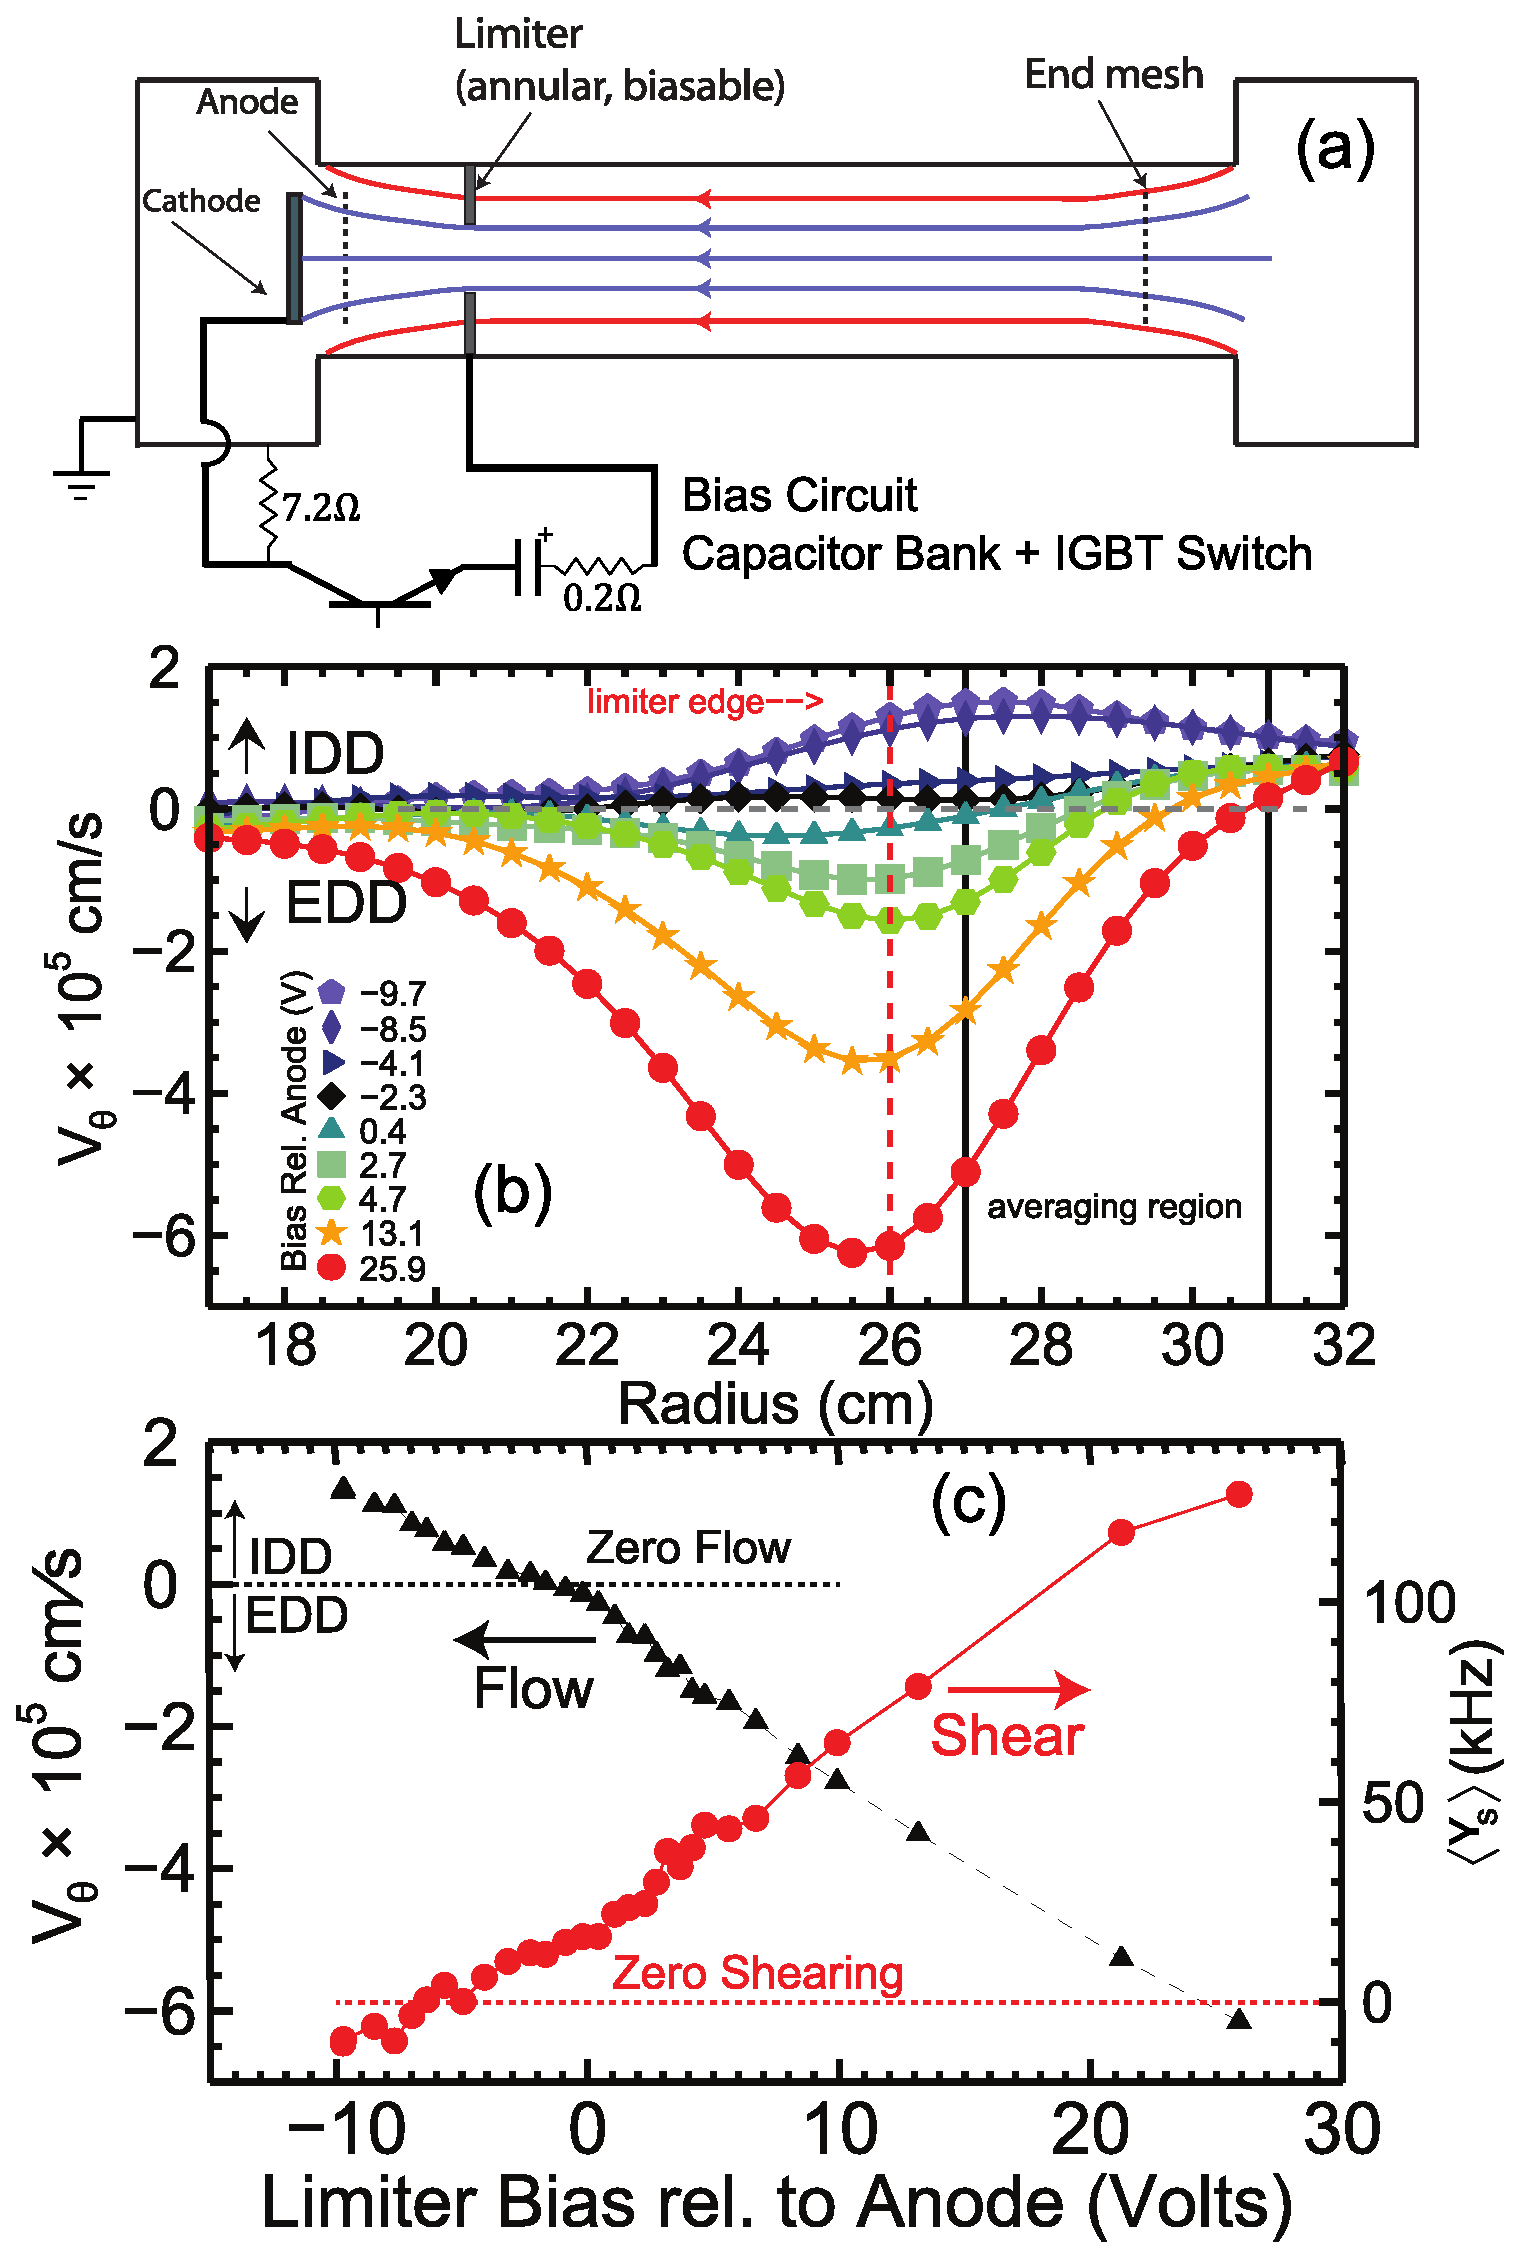
\includegraphics[width=8.5cm]{figure1.eps}}
\caption{\label{fig:velocity_flowshear} (a) Diagram of the LAPD device showing annular limiter.  (b) Velocity profiles using plasma potential from swept measurements. (c) Flow at the limiter edge (black, triangles) and mean shearing rate, averaged over $27 < r < 31$cm (red, circles).}
\end{figure}

The Large Plasma Device \cite{gek91} (LAPD) is a 17m long, $\sim$60cm diameter cylindrical plasma produced by a barium-oxide coated nickel cathode. In the experiments reported here, a plasma of density $\sim$$2 \times 10^{12}$ cm$^{-3}$ and peak temperature of ~8eV is produced in a uniform solenoidal magnetic field of 1000G.  Measurements of electron density, electron temperature, and potential (both plasma potential and floating potential) are made using Langmuir probes.   Measurements of ion saturation current ($I_{\rm sat} \propto n_e \sqrt{T_e}$) and floating potential ($V_f$) are taken with a 9-tip Langmuir probe (flush-mount tantalum tips) while temperature and plasma potential are determined using a swept Langmuir probe. $I_{\rm sat}$ fluctuations are taken as a proxy for density fluctuations for the measurements reported in this work. Density profiles are determined by scaling averaged $I_{\rm sat}$ profiles to line-averaged interferometer measurements of density.  Turbulent particle flux $\Gamma \propto \left<\tilde{n}_e \tilde{E}_\theta\right>$ is determined through correlating density fluctuations from one tip of this probe with azimuthal electric field fluctuations ($E_\theta$) derived from floating potential fluctuations on two azimuthally separated tips. Azimuthal $E\times B$ flow is computed using the swept-probe-derived plasma potential. 

A large annular aluminum limiter was installed in LAPD to provide a parallel boundary condition for the edge plasma and is biased relativeto the cathode of the plasma source to control plasma potential and cross-field flow.  The limiter is an iris-like design with four radially movable plates located 2.5m from the cathode as shown schematically in Fig.~\ref{fig:velocity_flowshear}(a).  The limiters create a 52cm diameter aperture; downstream of the limiter, plasma on field lines with radial location $r>26$cm has the limiter as a conducting end parallel boundary condition and plasma on field lines for $r<26$cm has the anode/cathode of the source region as a parallel boundary condition.  An electrically floating conducting end mesh terminates the plasma on the far end of the device.  A capacitor bank and transistor switch supply a voltage pulse to the limiter.  The bias pulse lasts 5ms during the flat-top of the $\sim$$15$ms plasmadischarge. The limiter is biased from $\sim$$10$V below to 50V above the anode potential.  Typically, plasma potential in the core LAPD plasma (plasma on field lines that connect to the source region) is very close to the anode voltage and the cathode sits near ground (vacuum chamber wall).  The anode potential is above the cathode potential by the discharge voltage, which was $\sim$$40$V during these experiments.

A recent experiment on the LAPD \cite{schaffner12} demonstrated the ability to achieve fine and continous control of steady-state azimuthal flow and flow shear through the use of biasable limiters. The spontaneous flow in the ion diamagnetic drift direction was first nullified and then reversed into the electron diamagnetic drift direction as bias was increased. This resulted in a continuous scan of flow shear states up to a shearing rate, $\gamma_s$, of about five times the turbulent inverse autocorrelation time  $\tau_{ac}^-1$ as measured in the unsheared state. Measurements of radial particle flux, density profiles and flutuation amplitude showed suppression of all three quantities as a function of normalized sheared flow. Figure ??? shows the experimental results for measurements of density fluctuation amplitude, ExB or radial velocity amplitude, crossphase, particle flux, radial correlation length, and diffusivity as a function of normalized shearing rate. The shearing rates achieved span two regimes: a weak-shear regime where $\gamma_{s}\tau_{ac} < 1$ and a strong-shear regime where $\gamma_{s}\tau_{ac} > 1$.

\section{Experimental Scaling}

\begin{figure}[!htbp]
\centerline{
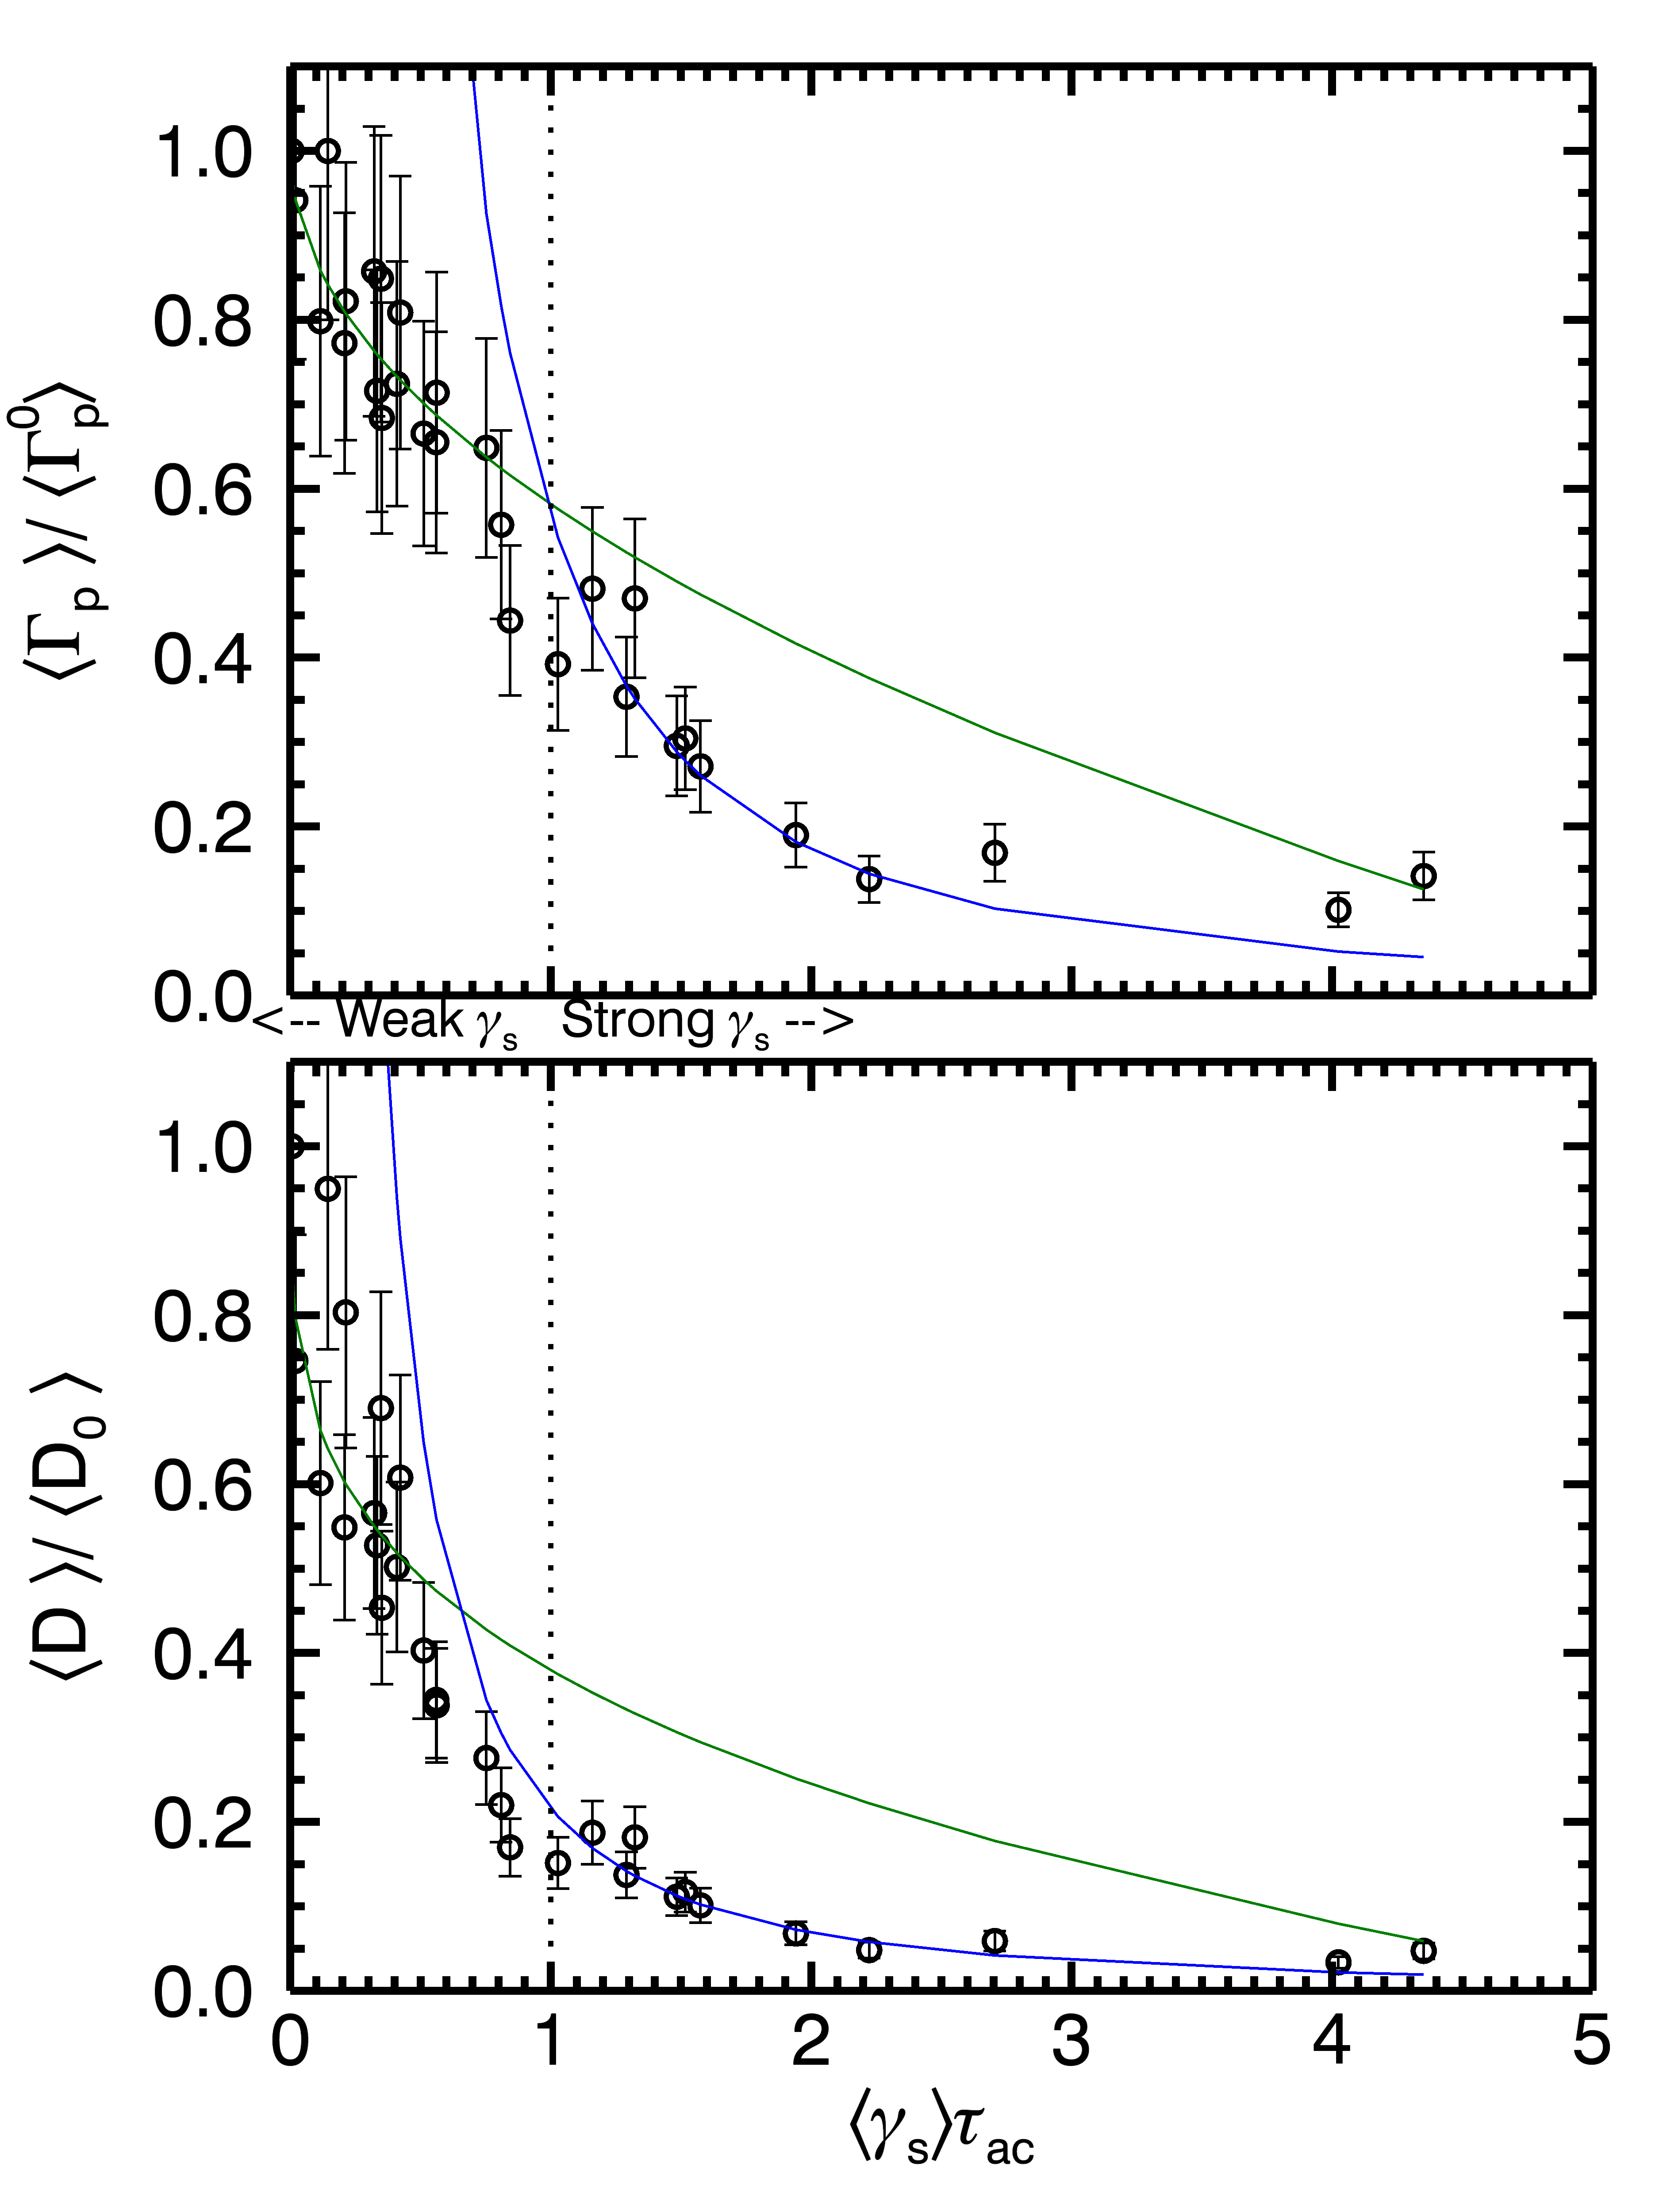
\includegraphics[width=8.5cm]{fluxandD}}
\caption{\label{fig:fluxandD} Scaling of (a)radial particle flux and (b)diffusion coefficient each normalized to the value at minimum shear, $\Gamma_{p}^{0} = 1.7\times10^{16} cm^{-2}$ and $D_{0} = 36.7 m^{2}/s$. The green curves correspond to $1-\gamma_{s}^{\nu}$ fits of the weak shear regime with $\nu = 0.501$ for flux and $\nu = 0.418$ for D. The blue curves correspond to $\gamma_{s}^{\nu}$ fits with $\nu = -1.719$ for flux and $\nu = -1.646$ for D.}
\end{figure}

\begin{figure}[!htbp]
\centerline{
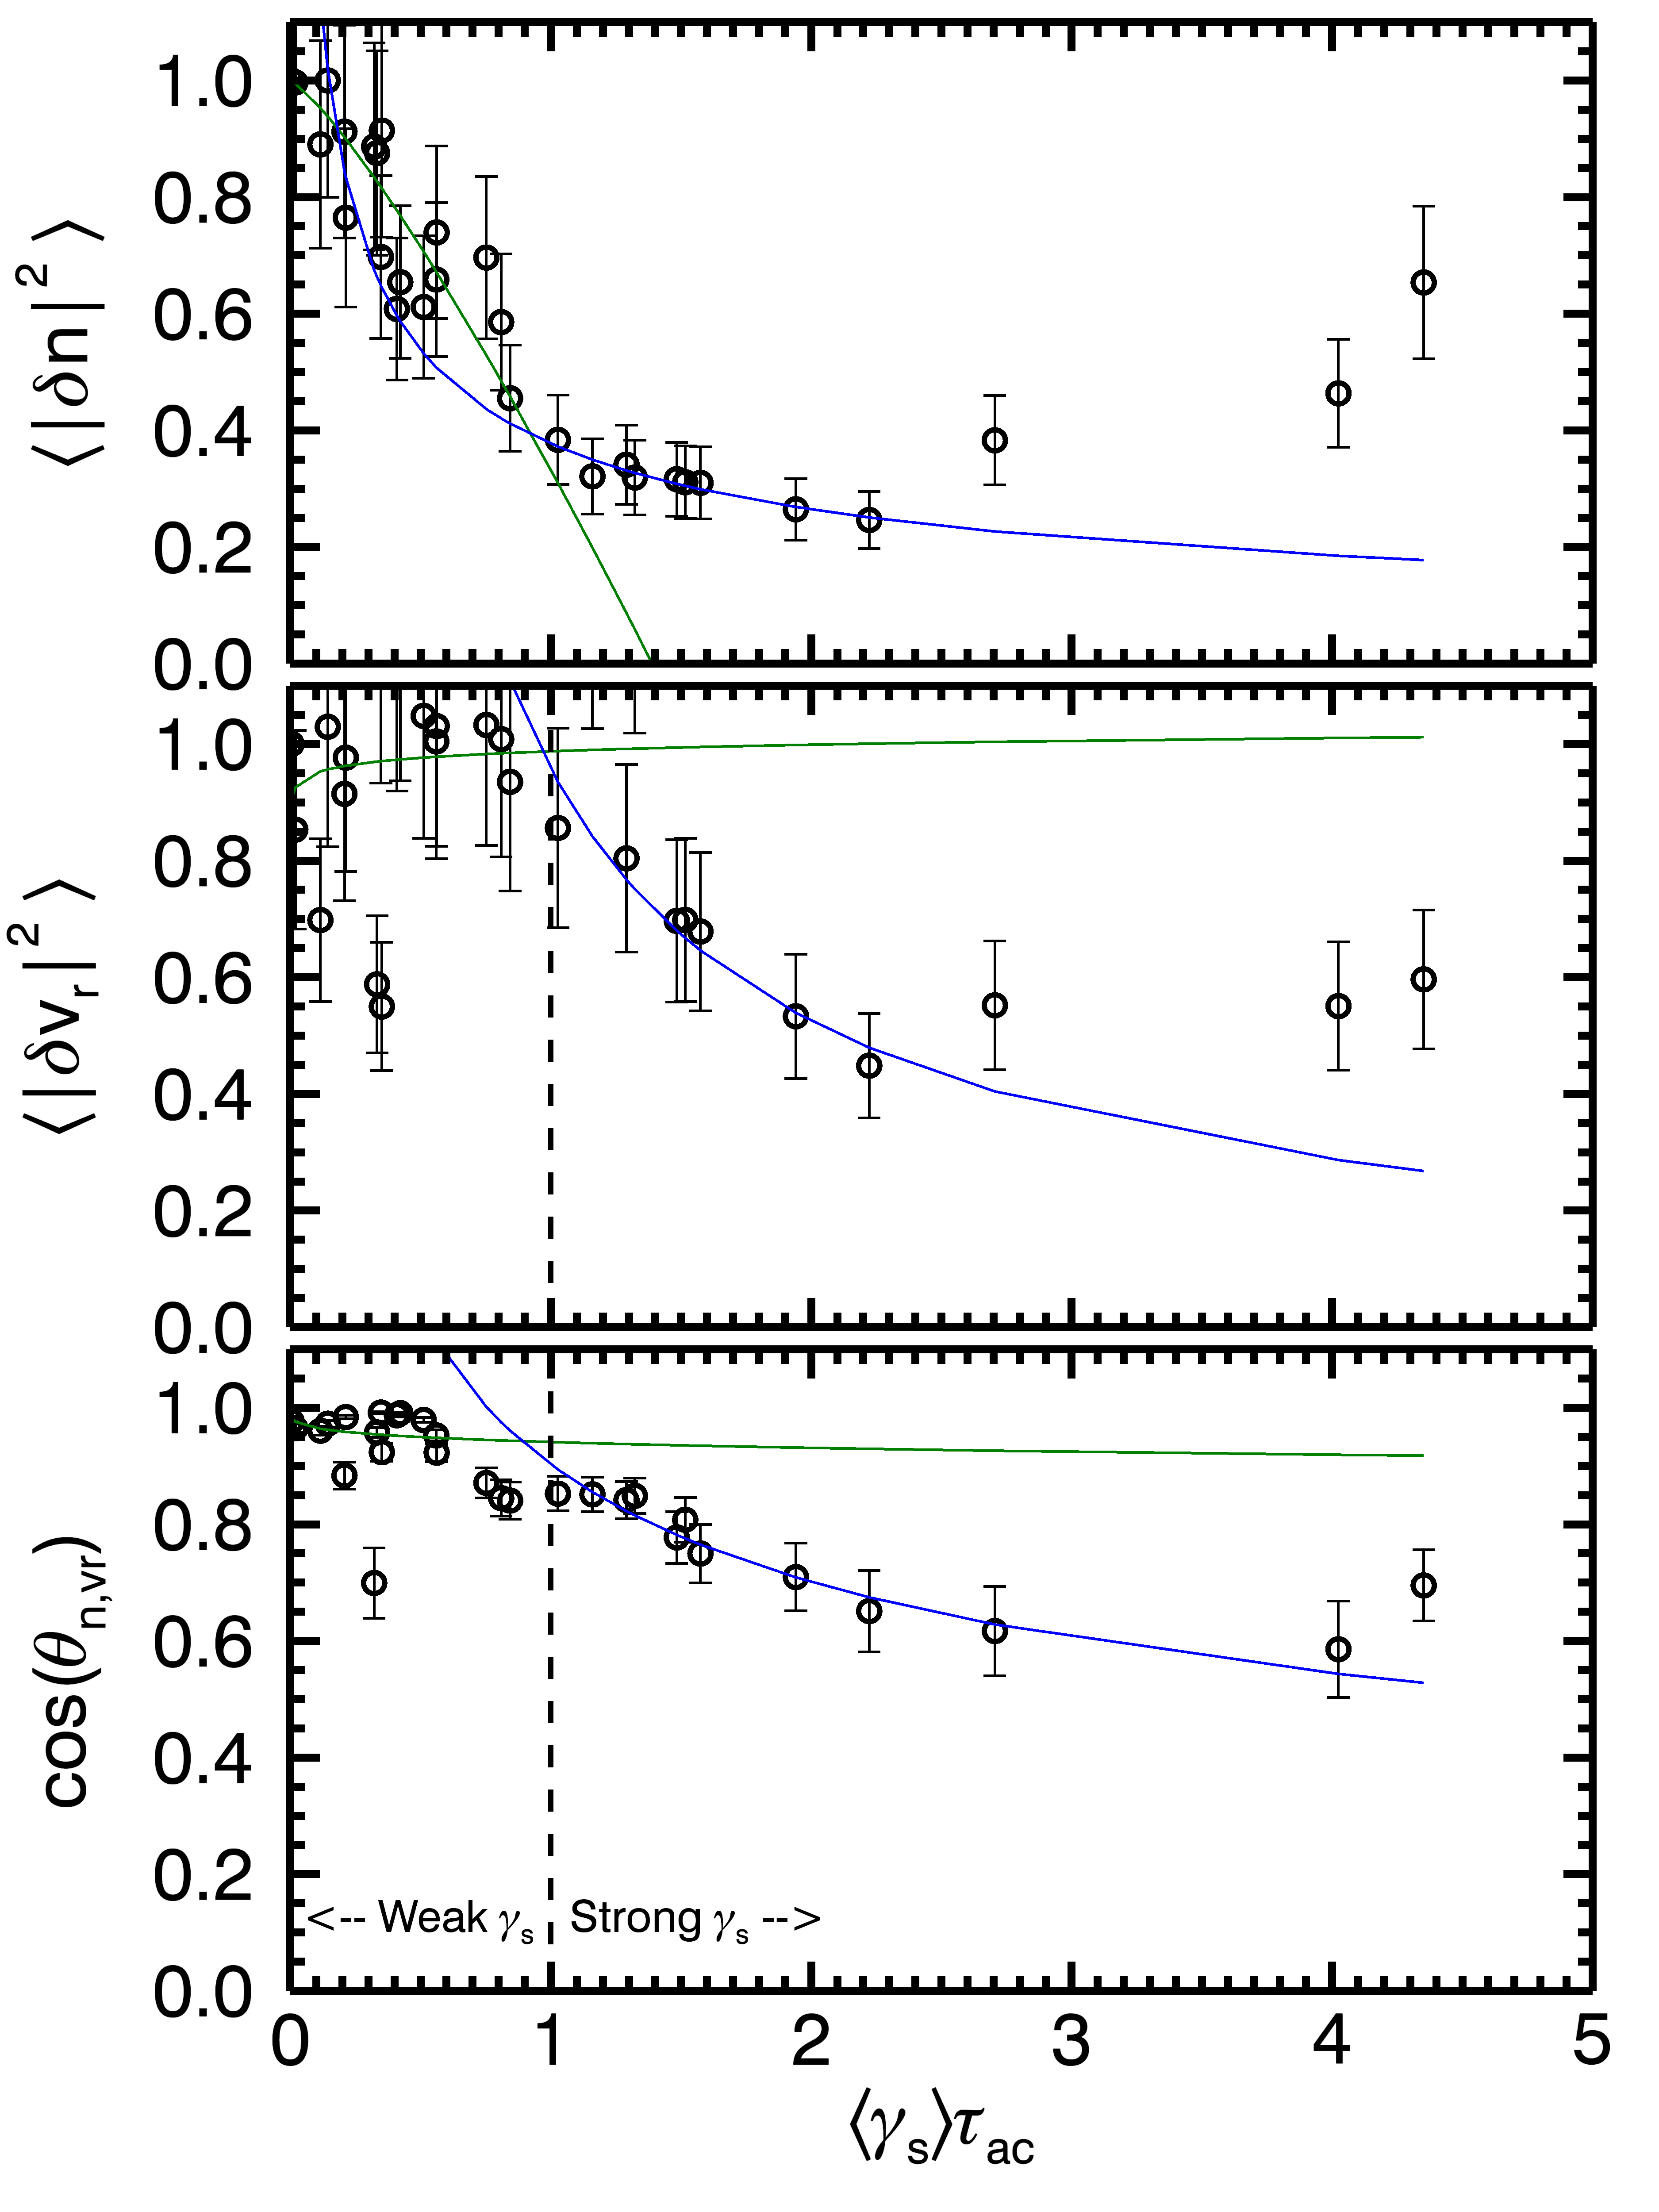
\includegraphics[width=8.5cm]{densvrcp}}
\caption{\label{fig:densvrcp} Scaling of (a)density fluctuation amplitude, (b)radial velocity fluctuation amplitude, and (c)relative crossphase between denisty and radial velocity fluctuations. Density and velocity fluctuation are each normalized to the value at minimum shear. The green curves correspond to $1-\gamma_{s}^{\nu}$ fits of the weak shear regime with $\nu = 0.501$ for flux and $\nu = 0.418$ for D. The blue curves correspond to $\gamma_{s}^{\nu}$ fits with $\nu = -1.719$ for flux and $\nu = -1.646$ for D.}
\end{figure}

\begin{figure}[!htbp]
\centerline{
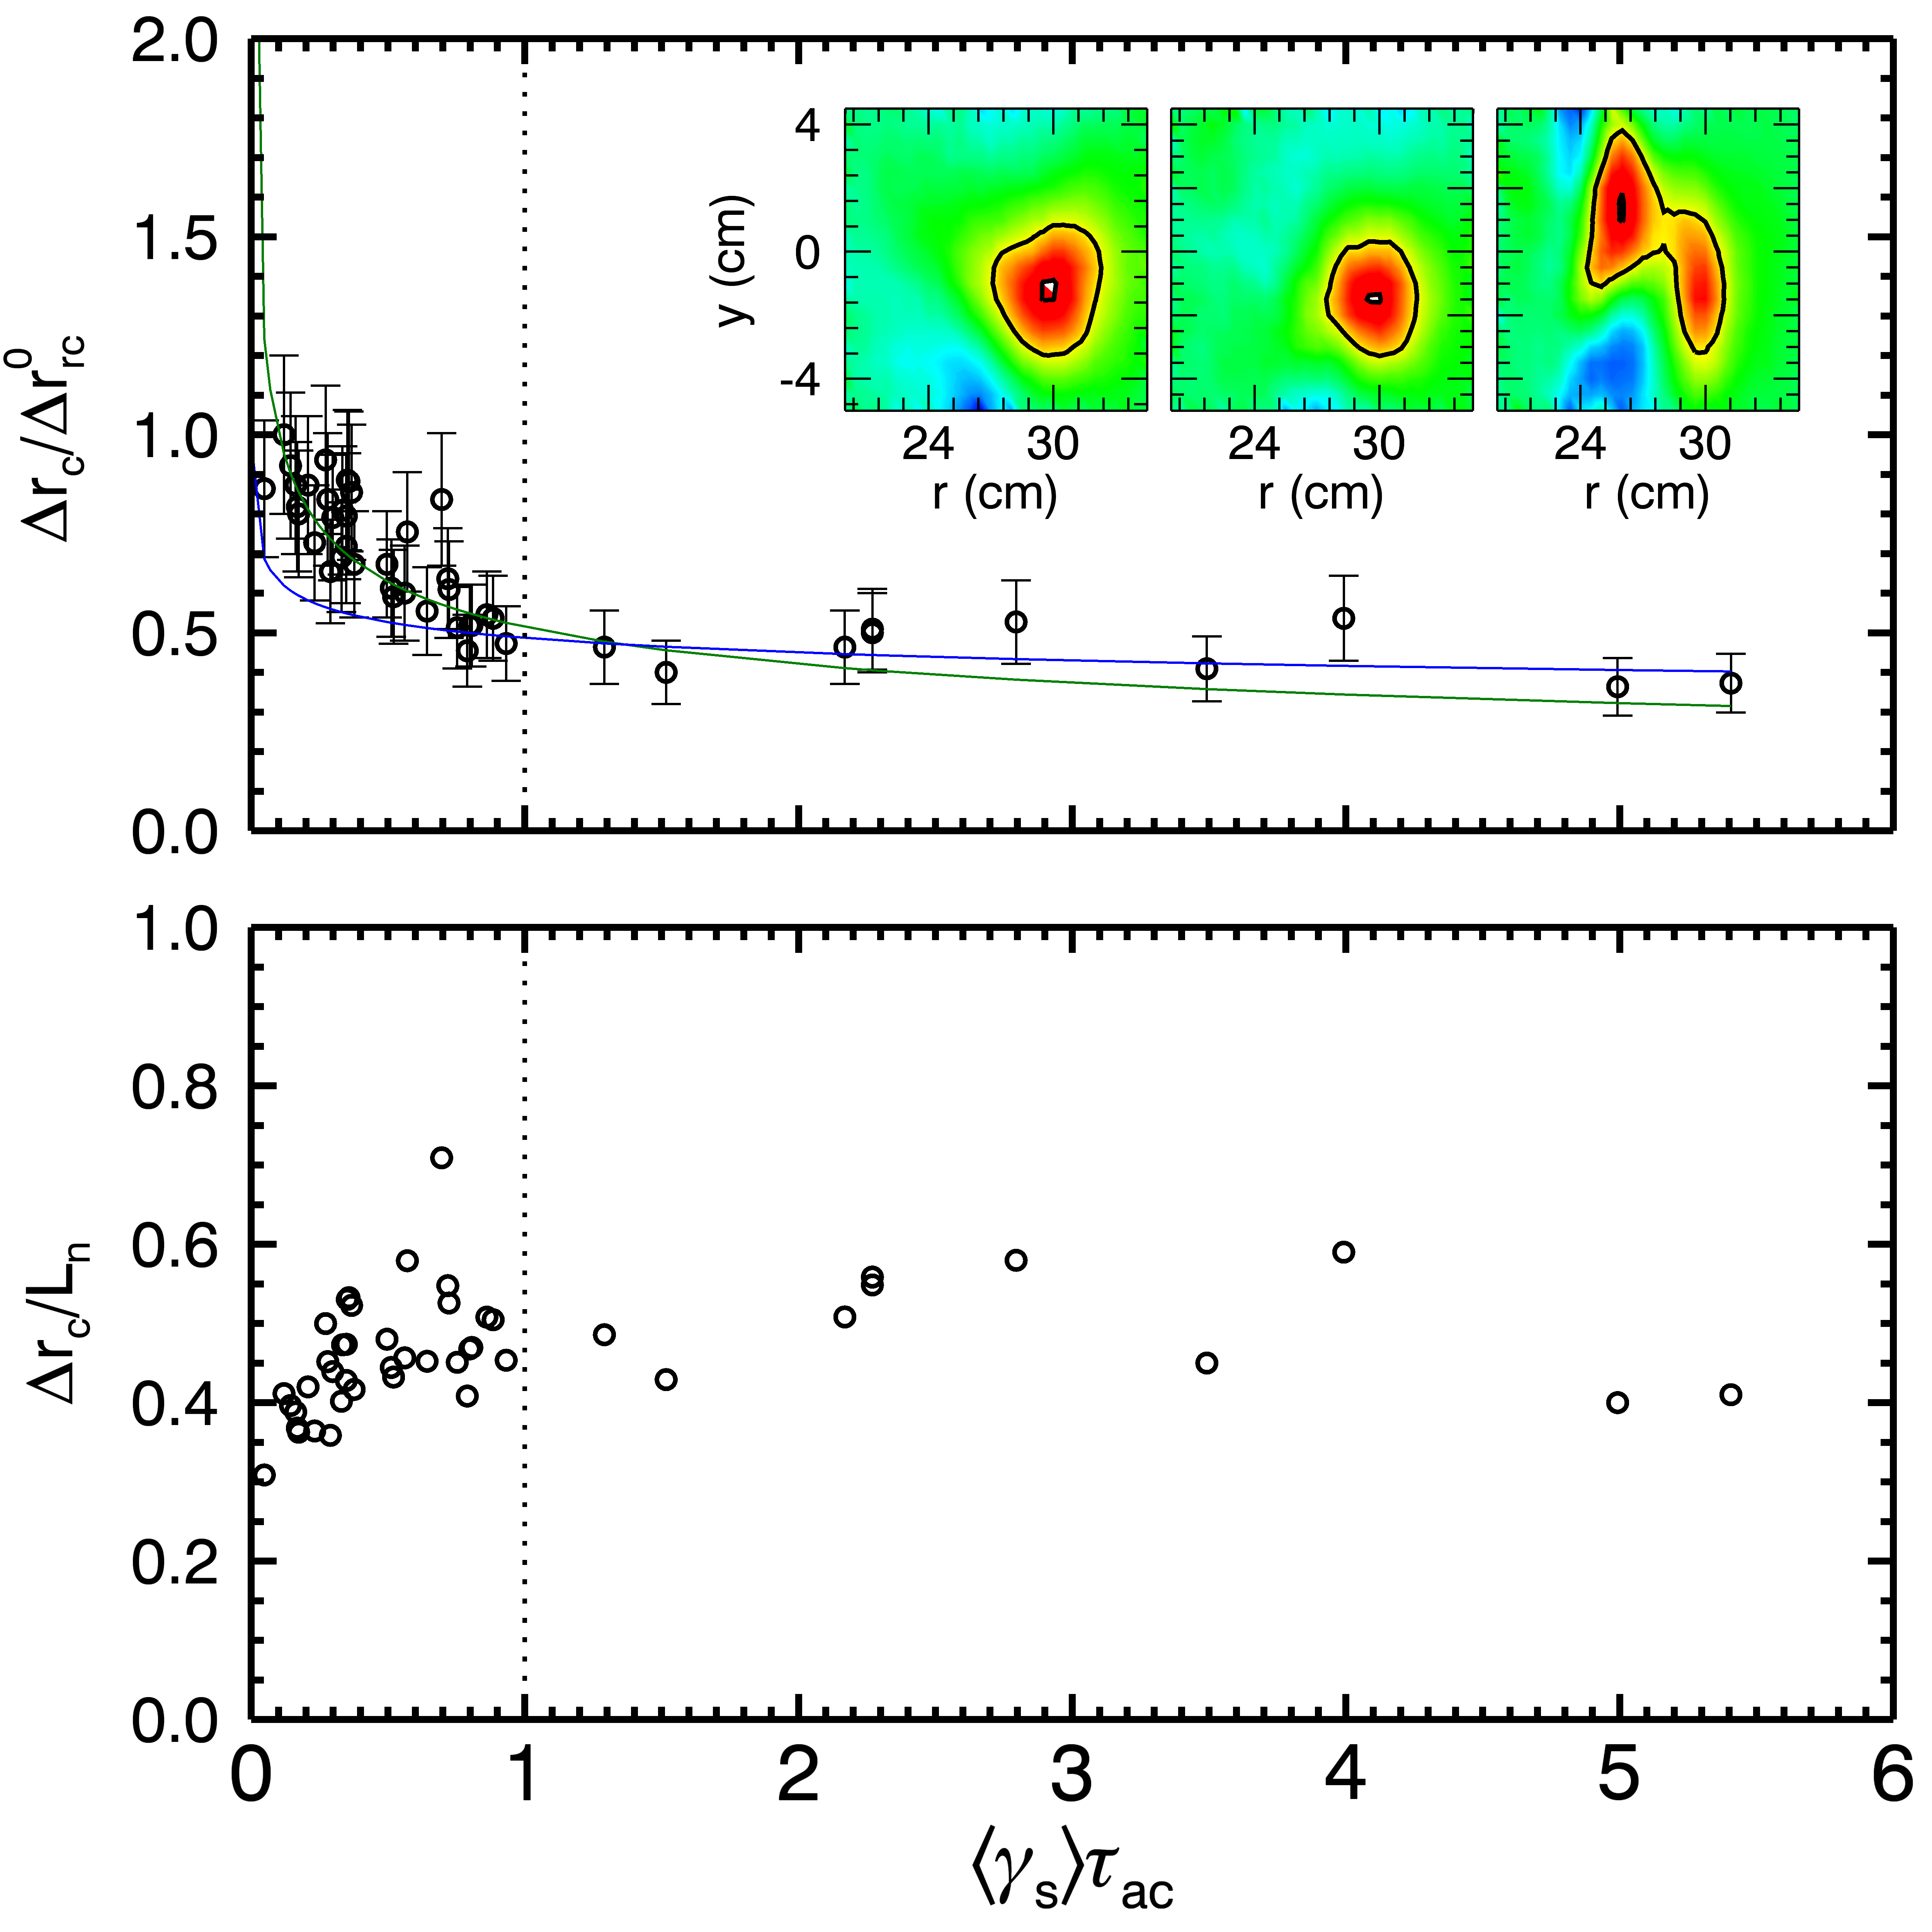
\includegraphics[width=8.5cm]{RadCorrLn}}
\caption{\label{fig:densvrcp} (a)Radial correlation length normalized to maximum correlation length versus normalized shearing rate with correlation planes of unbiased, zero shear, and high bias states in the inset. (b)Ratio of radial correlation length to density gradient scale length.}
\end{figure}

\begin{figure}[!htbp]
\centerline{
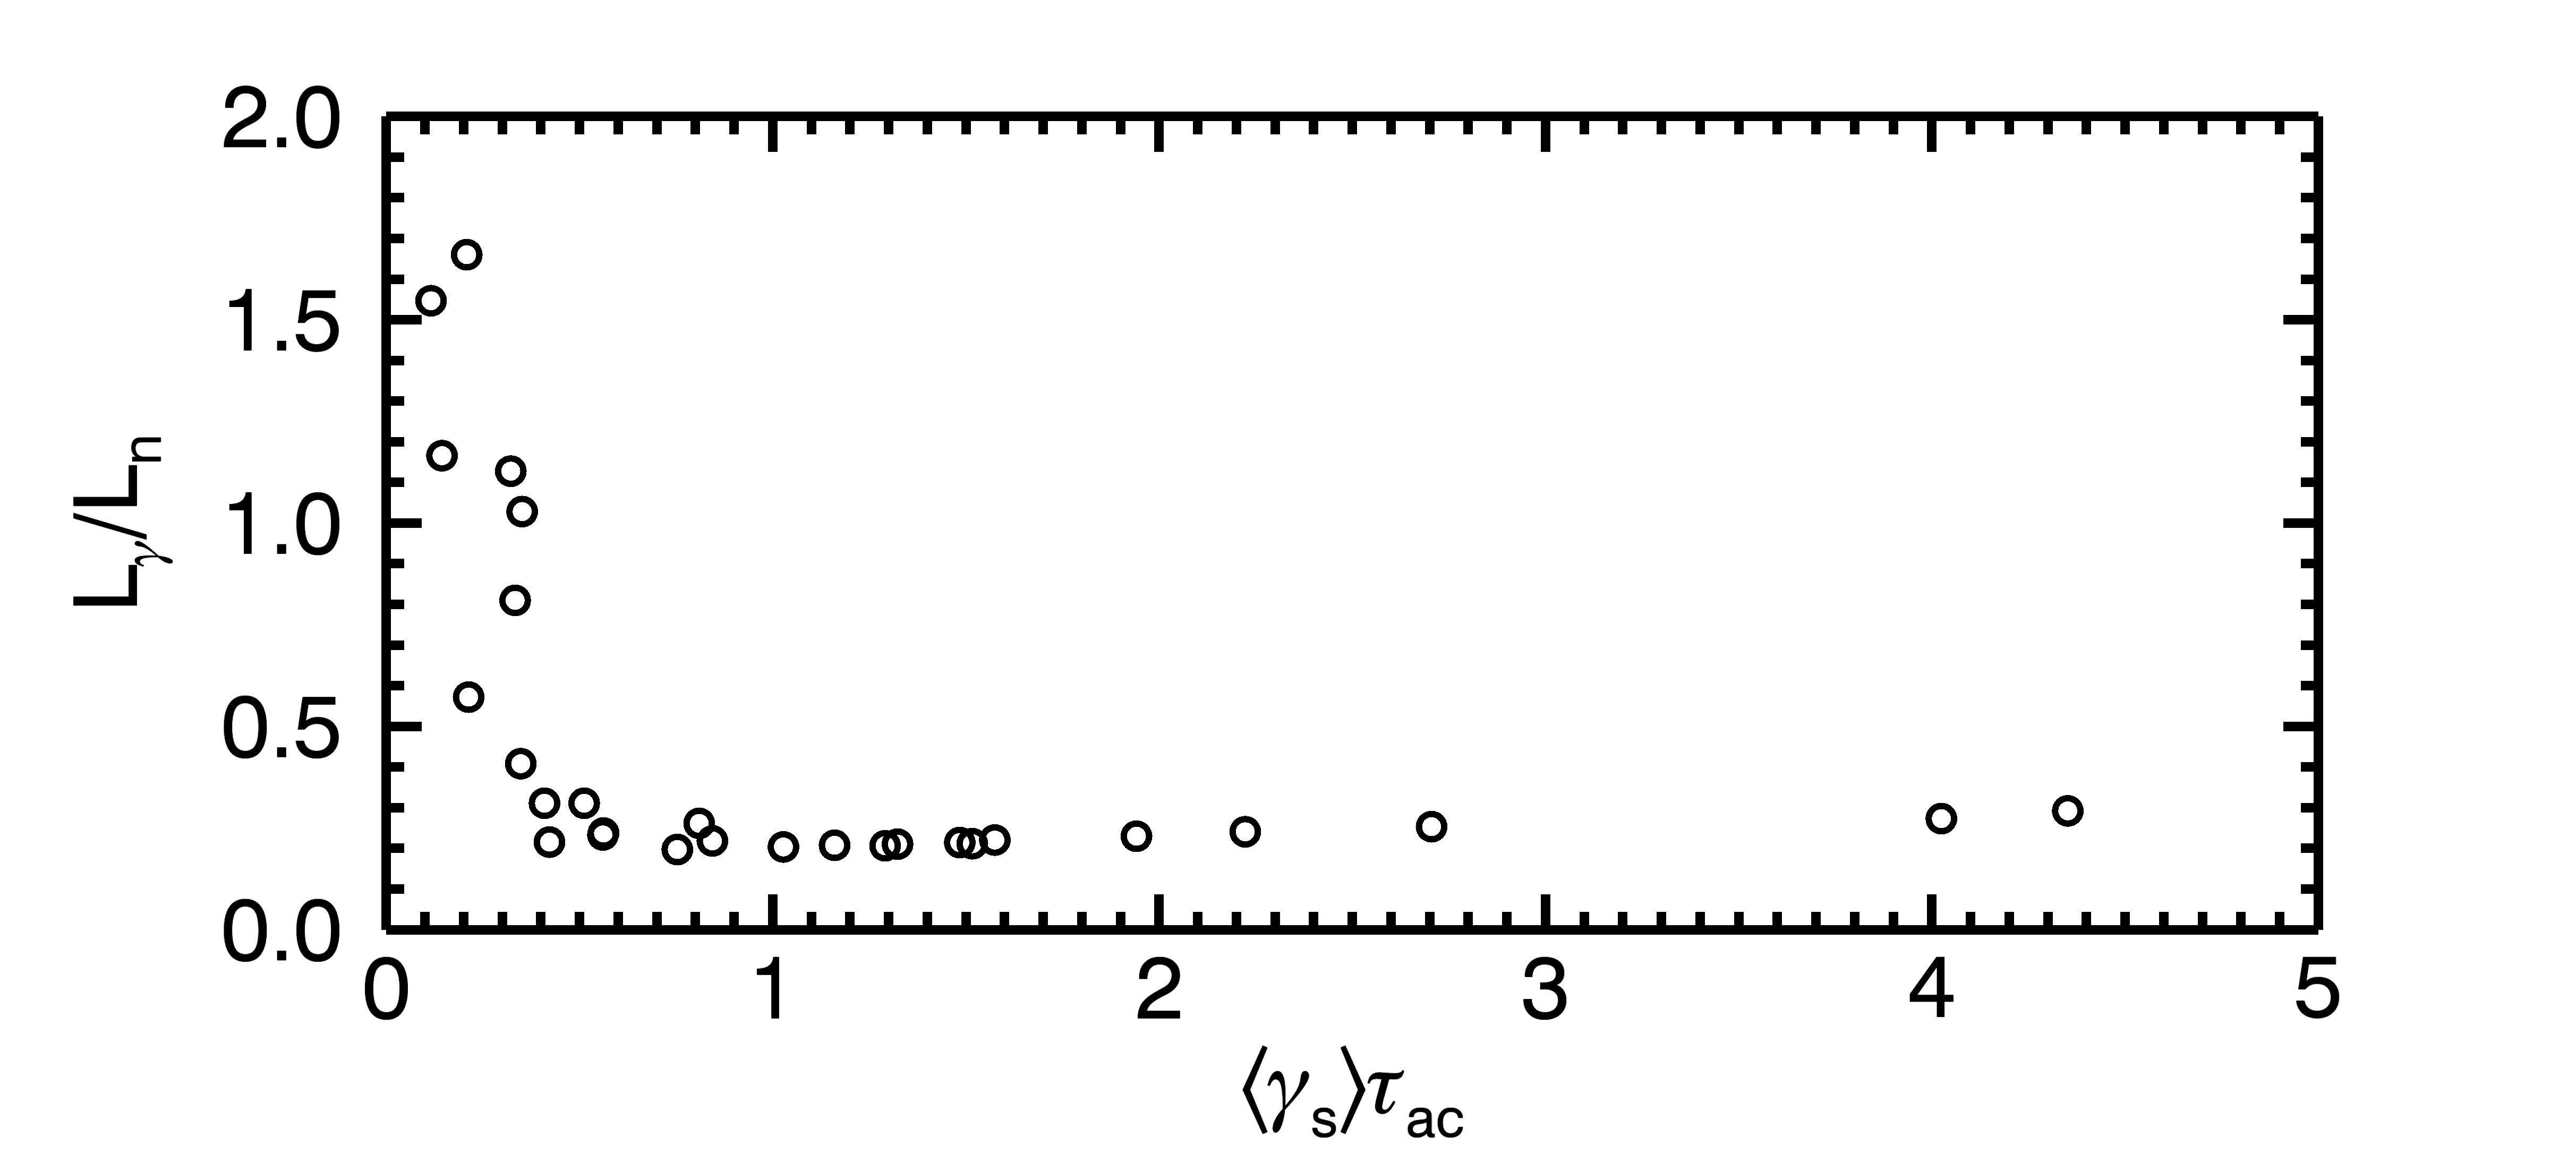
\includegraphics[width=8.5cm]{LgammaLn}}
\caption{\label{fig:LgammaLn} Ratio of shearing length scale to density gradient length scale versus normalized shearing in the radial region of 27 to 31cm.}
\end{figure}

\begin{table}
\caption{\label{tab:table1}Power-law fits for $|n(\textit{f})^{2}|$ scaling with shear for frequencies in 350Hz to 100kHz. Model form refers to how the shearing relates to the quantity in question, with C a constant and $\nu$ the power exponent.}
\begin{ruledtabular}
\begin{tabular}{llccc}
%One&Two&\mbox{Three}&\mbox{Four}&\mbox{Five}\\
Model form&$\gamma_{s}$ regime&$\nu$&$\chi^2$&$\chi^2/ndf$\\
\hline
$\sim 1-C\gamma_{s}^\nu$&$\gamma_{s}\tau_{ac}<1$&1.228&1.091&0.0642\\
$\sim 1-C\gamma_{s}^\nu$&$\gamma_{s}\tau_{ac}>1$&0.231&0.0332&0.0037\\
$\sim C\gamma_{s}^\nu$&$\gamma_{s}\tau_{ac}<1$&-0.116&0.1791&0.0094\\
$\sim C\gamma_{s}^\nu$&$\gamma_{s}\tau_{ac}>1$&-0.512&0.0024&0.0003\\
\end{tabular}
\end{ruledtabular}
\end{table}

\begin{table}
\caption{\label{tab:table2}Power-law fits for $|v_{r}(\textit{f})^{2}|$ scaling with shear for frequencies in 350Hz to 100kHz. Model form refers to how the shearing relates to the quantity in question, with C a constant and $\nu$ the power exponent.}
\begin{ruledtabular}
\begin{tabular}{llccc}
%One&Two&\mbox{Three}&\mbox{Four}&\mbox{Five}\\
Model form&$\gamma_{s}$ regime&$\nu$&$\chi^2$&$\chi^2/ndf$\\
\hline
$\sim C\gamma_{s}^\nu$&$\gamma_{s}\tau_{ac}<1$&0.016&0.2121&0.0117\\
$\sim C\gamma_{s}^\nu$&$\gamma_{s}\tau_{ac}>1$&-0.866&0.0037&0.0005\\
\end{tabular}
\end{ruledtabular}
\end{table}

\begin{table}
\caption{\label{tab:table3}Power-law fits for $\Gamma_{p}$ scaling with shear for frequencies in 350Hz to 100kHz. Model form refers to how the shearing relates to the quantity in question, with C a constant and $\nu$ the power exponent.}
\begin{ruledtabular}
\begin{tabular}{llccc}
%One&Two&\mbox{Three}&\mbox{Four}&\mbox{Five}\\
Model form&$\gamma_{s}$ regime&$\nu$&$\chi^2$&$\chi^2/ndf$\\
\hline
$\sim 1-C\gamma_{s}^\nu$&$\gamma_{s}\tau_{ac}<1$ &0.501   &0.332    &0.0189\\
$\sim 1-C\gamma_{s}^\nu$&$\gamma_{s}\tau_{ac}>1$ &0.638   &0.923    &0.1110\\
$\sim C\gamma_{s}^\nu$&$\gamma_{s}\tau_{ac}<1$   &-0.111  &0.146    &0.0077\\
$\sim C\gamma_{s}^\nu$&$\gamma_{s}\tau_{ac}>1$   &-1.719  &62.49    &5.2000\\
\end{tabular}
\end{ruledtabular}
\end{table}

\begin{table}
\caption{\label{tab:table4}Power-law fits for $cos(\theta_{nv_{r}})$ scaling with shear for frequencies in 350Hz to 100kHz. Model form refers to how the shearing relates to the quantity in question, with C a constant and $\nu$ the power exponent.}
\begin{ruledtabular}
\begin{tabular}{llccc}
%One&Two&\mbox{Three}&\mbox{Four}&\mbox{Five}\\
Model form&$\gamma_{s}$ regime&$\nu$&$\chi^2$&$\chi^2/ndf$\\
\hline
$\sim 1-C\gamma_{s}^\nu$&$\gamma_{s}\tau_{ac}<1$ &0.226   &6.1140    &0.3320\\
$\sim 1-C\gamma_{s}^\nu$&$\gamma_{s}\tau_{ac}>1$ &1.274   &0.0073    &0.0008\\
$\sim C\gamma_{s}^\nu$&$\gamma_{s}\tau_{ac}<1$   &-0.020  &0.0369    &0.0019\\
$\sim C\gamma_{s}^\nu$&$\gamma_{s}\tau_{ac}>1$   &-0.365  &0.0023    &0.0003\\
\end{tabular}
\end{ruledtabular}
\end{table}

\begin{table}
\caption{\label{tab:table5}Power-law fits for $D = \Gamma_{p}/\nabla{n}$ scaling with shear for frequencies in 350Hz to 100kHz. Model form refers to how the shearing relates to the quantity in question, with C a constant and $\nu$ the power exponent.}
\begin{ruledtabular}
\begin{tabular}{llccc}
%One&Two&\mbox{Three}&\mbox{Four}&\mbox{Five}\\
Model form&$\gamma_{s}$ regime&$\nu$&$\chi^2$&$\chi^2/ndf$\\
\hline
$\sim 1-C\gamma_{s}^\nu$&$\gamma_{s}\tau_{ac}<1$ &0.418   &1.4710    &0.0817\\
$\sim 1-C\gamma_{s}^\nu$&$\gamma_{s}\tau_{ac}>1$ &0.197   &0.0016    &0.0002\\
$\sim C\gamma_{s}^\nu$&$\gamma_{s}\tau_{ac}<1$   &-0.217  &0.4200    &0.0221\\
$\sim C\gamma_{s}^\nu$&$\gamma_{s}\tau_{ac}>1$   &-1.646  &0.0187    &0.0021\\
\end{tabular}
\end{ruledtabular}
\end{table}

\begin{table}
\caption{\label{tab:table6}Power-law fits for $\Delta r_{c}$ scaling with shear for frequencies in 350Hz to 100kHz. Model form refers to how the shearing relates to the quantity in question, with C a constant and $\nu$ the power exponent.}
\begin{ruledtabular}
\begin{tabular}{llccc}
%One&Two&\mbox{Three}&\mbox{Four}&\mbox{Five}\\
Model form&$\gamma_{s}$ regime&$\nu$&$\chi^2$&$\chi^2/ndf$\\
\hline
$\sim C\gamma_{s}^\nu$&$\gamma_{s}\tau_{ac}<1$ &-0.290 &5.8730 &0.1630\\
$\sim C\gamma_{s}^\nu$&$\gamma_{s}\tau_{ac}>1$ &-0.113 &3.7040 &0.3370\\
\end{tabular}
\end{ruledtabular}
\end{table}

The various experimentally measured quantities as functions of normalized shearing rate were fit to a power law in two ways reflecting in order to make comparisons to models of the form $1-\omega^{\nu}$ and those those of $\omega^{\nu}$. For the first model type, the measured quantity, y, was normalized to the value at zero shear, then transformed as $-(1-y)$. Then, taking the logrthim of both sides, a linear fit was made for points in the weak shear and in the strong shear separately. The resulting slope of the fit is taken as the power $\nu$. For the second type of model, no transformation of the quanitity y to $-(1-y)$ is made before the logrthms and fitting are taken. For a complete comparison to the wide range of model predictions made, fits were made for density fluctuation amplitude, radial particle flux, density-radial velocity fluctuation crossphase, radial velocity (ExB) fluctuation amplitude, radial correlation length, and experimental diffifusisivty ($\Gamma/\nabla n$). The best fits are summarized in Table 1 for each model type and for both weak and strong shear. The X2/ndf is also indicated in the tables.

\section{Discussion}











%In this letter, we report on the first experiments in which external control of flow is used to document the response of turbulence and transport to a continuous variation of flow shear, including a zero shear state and a reversal of the flow direction. Shearing rates ($\gamma_{s}= \partial V_{\theta}/\partial r$, where $V_{\theta} = E_r/B$) from zero to up to five times the turbulent autocorrelation rate measured at zero flow shear $(\tau_{ac}^{-1})$ are achieved. Turbulent particle flux is reduced with increasing shearing rate, regardless of the direction of the flow or sign of the flow shear, with significant reduction occuring for $\gamma_{s} \sim \tau_{ac}^{-1}$.  The observed reduction in particle flux is dominated by a decrease in low-frequency ($f < 10$kHz) density fluctuation amplitude. For low frequency fluctuations, the crossphase between density and azimuthal electric field fluctuations remain near zero for all shearing rates.  With higher shear ($\gamma_{s} > \tau_{ac}^{-1}$) we observe the emergence of a coherent mode localized spatially in the region of strong flow. Fluctuations from this mode appear to increase density fluctuations above 10kHz, but do not appear to contribute to particle flux.   

  
%Biasing experiments have been previously conducted on LAPD in which
%edge profile steepening and a reduction in turbulent flux was
%observed~\cite{maggs07,carter09}. In these experiments, edge flow was
%driven by biasing the vacuum chamber wall with respect to the
%plasma source cathode.  Transport reduction occurred only for biases
%above a threshold value.  Below the threshold, azimuthal flow was
%localized near the biased wall and no flow or flow shear was driven in
%the region where drift wave turbulence exists.  Above the threshold,
%the flow was able to penetrate radially inward; hence, strong flow and
%flow shear, with shearing rates far above the low-flow turbulent
%autocorrelation rate, was driven in the region of strong density
%gradient.   Recent experiments were successful in achieving more continuous control of potential and cross-field flow in the shadow of a small biased obstacle %inserted into the LAPD core plasma~\cite{zhou12}.  Both confinement improvement and degradation (formation of strong density depletions) were observed with the %density profile created by the obstacle in this case.  

%Motivated by the success of biasing obstacles to control flow, 


%\begin{figure}[!htbp]
%\centerline{
%\includegraphics[width=8.5cm]{plaspot.png}}
%\caption{\label{fig:velocity_flowshear}}
%\end{figure}


%The effect of biasing the limiters appears to manifest as a change in the plasma potential in the region radially beyond the limiter edge. Fig.~\ref{plaspot.png} shows radial profiles of plasma potential with respect to cathode potential as a function of increasing bias voltage. The anode voltage is indicated as well. The change in potential between the core region (set by the anode) and the limiter region (set by the biasing) results in an electric field in the region of the limiter edge. 

%Spontaneous azimuthal rotation of the LAPD plasma is observed when the limiters are
%unbiased (here the limiters are observed to float to a
%potential $\sim 10$V below the anode).  In this state, an edge flow
%(peaked just outside the limiter edge) is
%observed in the ion diamagnetic drift direction (IDD), as shown in
%Figure~\ref{fig:velocity_flowshear}(a).  Biasing the limiter positively
%with respect to the cathode tends to drive flow in the electron

%diamagnetic drift direction (EDD).  As the limiter bias is increased, the
%flow in the IDD is first reduced, then brought to separate near-zero flow
%and zero flow-shear states, and ultimately reversed with strong EDD flow.

%Measurements of profiles of density and particle flux
%were made for each bias flow state. Values are averaged over a range
%from $r=27$cm to $r=31$cm, a region where average flow and flow shear scale
%nearly linearly with limiter bias, as shown in
%Figure~\ref{fig:velocity_flowshear}(b).  All other spatially-averaged
%quantities shown in this paper are averaged over the same region in space.

%\begin{figure}[!htbp]
%\centerline{
%\includegraphics[width=8.5cm]{densprof}}
%\caption{\label{fig:densprof} Denisty profiles.}
%\end{figure}

%Fig.~\ref{fig:densprof} shows the density profiles for a range of limiter biases. It is obvious that as the bias reaches its highest values, the density gradient is signficantly steepened. Less obvious, but definitely important is that the profile begins in a slightly steeped state (black) but then begins to shallow out when the limiter bias approaches the anode bias (red) before showing significant steepening in the high bias region. This change can be quantified by calculating the average denssity gradient length scale the radial region indicated.

%\begin{figure}[!htbp]
%\centerline{
%\includegraphics[width=8.5cm]{figure2.eps}}
%\caption{\label{fig:densgrad} Density gradient length scale versus limiter bias. Inset shows density profile at three bias values.}
%\end{figure}

%Figure~\ref{fig:densgrad} shows the variation in the spatially-averaged density gradient length scale, $L_{n} = \lvert \nabla \ln n \rvert ^{-1}$ with
%increasing limiter bias.  As the limiter bias is increased, reducing
%the IDD flow, an increase in the gradient scale length is observed,
%indicating a degradation of radial particle confinement. The gradient scale length peaks
%when the averaged shearing rate is near zero. As the bias is
%increased further, reversing the flow and again increasing the
%shearing rate, the gradient gradually steepens and the
%scale length is lowered, indicating improved radial particle confinement.  

%\begin{figure}[!htbp]
%\centerline{
%\includegraphics[width=8.5cm]{figure3.eps}}
%\caption{\label{fig:sheargradflux} (a)Gradient scale length versus shearing rate. (b)Particle flux normalized to no-shear
%  flux as a function of normalized shearing rate. Filled symbols
%  represent points with flow in the IDD. Inset: Measured turbulent particle flux versus
%  gradient scale length.}
%\end{figure}

%The observed variation of $\langle L_{n} \rangle$ with bias is best
%organized when compared to the shearing rate, $\gamma_{s}$, as is
%shown in Figure~\ref{fig:sheargradflux}(a).   The shearing rate is
%normalized to the autocorrelation rate of density fluctuations
%measured in the zero-shear state.  An autocorrelation rate of $\tau_{ac}^{-1} \approx $ 28kHz $(\tau_{ac} \approx 36\mu s)$ is calculated by taking the %half-width at half-maximum of a Hilbert transform of the $I_{\rm sat}$
%autocorrelation function.  Confinement improvement (decreased $\langle
%L_n \rangle$) occurs continuously and gradually with increasing
%$\gamma_{s}$ and reaches saturation for $\gamma_{s} \approx \tau_{ac}^{-1}$ (a normalized $\gamma_{s}$ of 1).  The profile steepening
%appears to be largely independent of the direction of the flow (or radial electric field): IDD (filled points) and EDD (open points) flow cases follow the same trend when plotted against normalized shearing rate.

%Conversely, the scale length changes do not line up along a single curve if compared to flow rather than flow shear. Fig~\ref{fig:Lnvsflow} shows the same quantities of scale length versus the flow measured at the limiter edge for each bias. Points around the flow minimum are not symmetric; this is physically due to the fact that the minimum shearing rate does not coincide with the minimum flow point. Fortunately this difference allows us to observe the fact that is is flow shear, not necessarily flow, that establishes a maximual density gradient, or minimal confinement.

%Measured changes in turbulence and turbulent particle flux are
%consistent with the observed changes in the density profile.  The
%turbulent particle flux can be written\cite{powers74}:
%\begin{equation}
%\Gamma = \frac{2}{B} \int^{\infty}_{0} \lvert n(f) \rvert \lvert E_{\theta}(f) \rvert \gamma_{(n,E_{\theta})}(f) \cos [\phi_{(n,E_{\theta})}(f)] df
%\label{eq:fluxint}
%\end{equation}
%where $n(f)$ and $E_\theta(f)$ are the Fourier transforms of
%the density and azimuthal electric field fluctuations;
%$\gamma_{(n,E_\theta)}$ is the coherency between density and electric
%field; and $\phi_{(n,E_\theta)}$ is the cross-phase angle between
%density and electric field.

%Fig~\ref{fig:particlefluxprofiles} shows profiles of these particle flux for varying bias states. The natural state represented by the black curve shows that measured flux peaks in the region of density gradient. As bias is increased, shearing increases and both peak and overall flux increases reaching a maximum at bias 7. Beyond this bias, the flux is generally decreased across the entire radius except for a very narrow region just inside the limiter edge.

%\begin{figure}[!htbp]
%\centerline{
%\includegraphics[width=8.5cm]{particlefluxprofiles.png}}
%\caption{\label{fig:particlefluxprofiles}}
%\end{figure}

%In Figure~\ref{fig:sheargradflux}(b) shows the spatially-averaged turbulent
%particle flux as a function of normalized shearing rate.  The
%turbulent flux decreases continuously with increasing shearing rate;
%however the observed decrease is slightly slower than that observed
%for $L_n$.  The inset in Figure~\ref{fig:sheargradflux}(b) shows that the variation in
%turbulent flux is correlated with the changes in $L_n$ (but scales in a way
%that is inconsistent with Fick's law using a fixed diffusion coefficient).  The
%trend in reduced particle flux is the same for either direction of
%flow (IDD or EDD).  The cause for the reduction in turbulent particle
%flux can be explored by considering individual terms in the integrand
%of Eqn.~\ref{eq:fluxint}.

%Density fluctuations were reduced significantly with increasing
%shearing in these experiments.  Figure~\ref{fig:powercontour}(a) shows
%changes in the spatially-averaged density fluctuation spectrum
%with shearing rate.  The shearing rate is signed in this figure, and
%negative shearing rates occur for flow in the IDD. Most of the power
%is located in frequencies $<10$kHz and in this range, power decreases
%overall with increasing shearing rate.  A decrease of about one order
%of magnitude in fluctuation power is seen between the minimum shear
%state and the high shear regime where $L_n$ and particle flux are
%minimized; this is made clearer in Figure~\ref{fig:powercontour}(b).  At
%higher shearing rates, $\gamma_{s} \gtrsim \tau_{ac}^{-1}$, a coherent

%mode emerges.  The frequency of the mode increases with shearing rate
%and the fluctuation amplitude is localized to the peak of the
%azimuthal flow.

%\begin{figure}[!htbp]
%\centerline{
%\includegraphics[width=8.5cm]{figure4.eps}}
%\caption{\label{fig:powercontour} (a) Contour plot of log $I_{\rm sat}$/density fluctuation power versus shearing rate and frequency. (b) Power spectra for four %different values of shearing rate.}
%\end{figure}

%Figure~\ref{fig:fluxcomps}(a) shows the reduction in total density fluctuation amplitude with shear in two frequency bands: all frequencies below 100kHz in black and all frequencies above 10kHz in red. With the emergence of the coherent mode, the
%high frequency fluctuation amplitude does show an increasing trend at higher shearing
%rates but there is a strong overall decrease in fluctuation amplitude with shearing.
%A reduction is also seen in $E_\theta$ fluctuation amplitude, as shown in
%Figure~\ref{fig:fluxcomps}(b); however this reduction is weaker than
%observed in density fluctuations.  The cross-phase between
%$n$ and $E_\theta$ does not change significantly with
%shearing. As shown in Figure~\ref{fig:fluxcomps},
%$\cos[\phi_{(n,E_\theta)}] \sim 1$ for all shearing rates.  For
%higher frequencies ($f > 10$kHz), the cross-phase does change with
%shearing, with $\cos[\phi_{(n,E_\theta)}]$ trending toward zero at
%higher shear.  This crossphase change explains why the coherent mode
%that emerges at higher shearing rate does not contribute to an
%increase in the particle flux.  The coherency between $n$ and
%$E_\theta$ also decreases with shearing rate, as shown in 
%Figure~\ref{fig:fluxcomps}.  Overall, the decrease in flux is primarily
%due to a decrease in turbulent amplitude.  This observation is distinct from previous work with flows driven by vacuum-chamber-wall
%biasing on LAPD. In those experiments, turbulent amplitude decreased little while the
%turbulent cross-phase experienced a significant change, leading to
%reduced particle flux~\cite{carter09}.  In the experiments reported
%here, the magnetic field is higher (1000G versus 400G) and normalized
%shearing rates are lower (near unity).  Cross-phase change is expected
%in cases with very strong shearing ($\gamma_{s} \gg \tau_{ac}^{-1}$)~\cite{terry01}.  Future experiments will explore the
%variation of the turbulent response to higher normalized shearing
%through changing plasma parameters, in particular magnetic field.  

%\begin{figure}[!htbp]
%\centerline{
%\includegraphics[width=8.5cm]{figure5.eps}}
%\caption{\label{fig:fluxcomps} Components of particle flux versus shearing rate including $I_{\rm sat}$/density fluctuation power(a), electric field fluctuation %power(b), crossphase(c) and coherency(d) with black points for low or all frequency, red for high only.}
%\end{figure}


%\section{Correlation Planes}

%Some theories suggest that flow shear is expected to produce radial decorrelation of turbulence,
%breaking up turbulent eddies into smaller radial scales which in turn results in decreased turbulent fluctuations~\cite{biglari90}.
%We measure the radial correlation length in the plane of the plasma by computing a two-dimensional turbulent correlation functions sing
%two probes: one probe is held fixed in space (phase reference) and
%correlating its signals against a second probe, axially separated
%from the first, which is moved shot-to-shot in a plane perpendicular
%to the magnetic field.  The radial correlation length, $\Delta r_c$,
%is derived from the radial width of the Hilbert transform of the
%correlation function (half-radial-width and half-maximum at the
%location of peak correlation). We can just as easily extract a correlation length in the y-diretion, representing the extent in the azimuthal direction. This %length can be used for calculating an estimate of the azimuthal wavenumber, $k_{\theta}$, as well as the azimuthal mode number, M.

%Fig.~\ref{fig:corrplanes} shows the cross-correlation contour plot for three shearing regimes---a)unbiased, IDD flow, b)no-shear, c)high flow/shear---normalized %to the maximum correlation within each regime. The reference tip is located at 30cm, just beyond the edge of the limiter and within the spatial averaging region. %The most striking change occurs between the no-shear state and a high shear state; the correlation function shifts from a fairly circular shape to radially narrowed and azimuthally elongated structure. In the high bias case, a series of structures can be seen located directly at the limiter edge. This is believed to be a mode-pattern caused by the mode that appears at high bias. Fig.~\ref{fig:filteredhighbias} shows the same correlation plane but with the frequencies at which the mode is observed removed leaving the correlation structure unaffected.

%\begin{figure}[!htbp]
%\centerline{
%\includegraphics[width=8.5cm]{corrplanes.png}}
%\caption{\label{fig:corrplanes} }
%\end{figure}

%\begin{figure}[!htbp]
%\centerline{
%\includegraphics[width=8.5cm]{radcorr}}
%\caption{\label{fig:filteredhighbias} }
%\end{figure}

%Accumulating radial correlation lengths from correlation functions at various shearing states, it can be shown that the radial correlation length 
%decreases with increasing shearing, as shown in
%Fig.~\ref{fig:radcorr}.

%Discuss rad correlation length vs grad scale length

%At higher shearing rate, a coherent mode
%pattern appears (as shown in the rightmost inset plot) in addition to
%the primary correlation peak (the coherent mode is
%pattern shifted inward of the reference probe location which was $r=30$cm).  The coherent
%mode does lead to an increasing trend in the radial correlation length
%at higher shear, but the overall trend is a substantial reduction
%($\gtrsim 2$) in the radial correlation length from the no shear state.

%\begin{figure}[!htbp]
%\centerline{
%\includegraphics[width=8.5cm]{radcorr}}
%\caption{\label{fig:radcorr} $\Delta r_{c}$ with
%  reference probes at 28,29,30,31 or 32cm with $\gamma_{s}$ averaged over measured $\Delta r_{c}$.  Inset shows 2D correlation
%  structure for 3 cases: unbiased (spontaneous flow), minimum flow
%  shear and strong EDD flow.}
%\end{figure}


%\section{Comparison to Theory}

%Various theories have been proposed and elaborated as to the quantitative effect of flow shear on fluctuations levels as well as particle flux. Given the fine resultion of this dataset in both weak and strong shearing regimes, a comparison to these various theories can be made. A summary of the various theories is presented.

%BDT says shear^(-2/3) scaling for fluctuations
%Shiang says shear^(-2); updated by Zhang and Mahajan to be 1-(1/shear^2) for low shear, shear^(-2) for arbitrary shear and shear^(-2/3) if Diffusion coeffiect, %D, is insensitive to turbulence.

%Ware extended the study to flux suggesting that particle flux $\sim$ shear^(-2) while Terry 01 says that flux decrease with 1/shear for amplitude and 1/shear^3 %for crossphase 

%Lastly, we add a comparison of our data to a simple theory, the
%Biglari-Diamond-Terry (BDT) model~\cite{biglari90}, which predicts a
%power-law scaling with shearing rate of the turbulent
%amplitude of the form: $\left(\gamma_{s}/\tau_{ac}^{-1}\right)^{-\alpha}$. As seen in
%Figure~\ref{fig:fluxcomps}, a best fit of $\alpha = 0.530$ compares
%favorably to the BDT prediction of $\alpha = 2/3$ for the reduction in
%density fluctuation amplitude. 
%It should be noted, however, that the
%BDT model is fairly simple and the validity of its assumptions is
%questionable for the experimental conditions reported here.  In
%particular, as the shearing rate is increased in LAPD, the density
%profile is changing (in BDT a fixed drive is considered).  Future work
%will focus on direct comparisons to more comprehensive models of shear
%suppression, including comparisons to two-fluid simulations using the
%BOUT++ 3D turbulence code~\cite{umansky11}.  

%This letter presents the first experiments in which the response of
%pressure-gradient-driven turbulence to a continuous
%variation of shearing rate, including a near-zero flow shear state and
%a reversal in the direction of flow, is studied.  Increased shearing
%improves radial particle confinement regardless of the direction of
%the azimuthal flow or sign of the flow shear. The observed reduction of
%turbulent particle flux with shear is attributed to a reduction in the
%amplitude of density fluctuations. These
%experiments were performed at a fixed set of plasma parameters (fixed
%magnetic field, neutral pressure, discharge power); future work will
%explore the variation in turbulent response to shear as these
%parameters are varied.  

\providecommand{\noopsort}[1]{}\providecommand{\singleletter}[1]{#1}%
\begin{thebibliography}{10}

\bibitem{schaffner12}
D.A. Schaffner {\it et~al.}, Phys. Rev. Lett. {\bf 109}, 135002 (2012).

\bibitem{burrell97}
K. Burrell, Phys. Plasmas {\bf 4},  1499  (1997).

\bibitem{terry00}
P. Terry, Rev. Mod. Phys. {\bf 72},  109  (2000).

\bibitem{wagner82}
F. Wagner {\it et~al.}, Phys. Rev. Lett. {\bf 49},  1408  (1982).

\bibitem{taylor89}
R. Taylor {\it et~al.}, Phys. Rev. Lett. {\bf 63},  2365  (1989).

\bibitem{weynants92}
R. Weynants {\it et~al.}, Nucl. Fusion {\bf 32},  837  (1992).

\bibitem{boedo00}
J. Boedo {\it et~al.}, Nucl. Fusion {\bf 40},  7  (2000).

\bibitem{silva06}
C. Silva {\it et~al.}, Plas. Phys. Control Fusion {\bf 48},  727  (2006).

\bibitem{sakai93}
O. Sakai and Y. Yasaka and R. Itatani, Phys. Rev. Lett. {\bf 70},  4071 (1993).

\bibitem{maggs07}
J. Maggs {\it et~al.}, Phys. Plasmas {\bf 14},  052507  (2007).

\bibitem{carter09}
T. Carter and J. Maggs, Phys. Plasmas {\bf 16},  012304  (2009).

\bibitem{burrell99}
K. Burrell, Phys. Plasmas {\bf 6},  12  (1999).

\bibitem{tynan09}
G. Tynan {\it et~al.}, Plasma Phys. Control Fusion {\bf 51}, 113001  (2009).

\bibitem{biglari90}
H. Biglari {\it et~al.}, Phys. Fluids B. {\bf 2},  1  (1990).

\bibitem{kim04}
E.-J. Kim {\it et~al.}, Phys. Plasmas {\bf 11},  10  (2004).

\bibitem{ware96}
A. Ware {\it et~al.}, Plasma Phys. Control Fusion
  {\bf 38},  1343  (1996).

\bibitem{amatucci96}
W.E. Amatucci {\it et~al.}, Phys. Rev. Lett. {\bf 77},  1978  (1996).

\bibitem{jass72}
D. Jassby, Phys. Fluids {\bf 15},  9  (1972).

\bibitem{gek91}
W. Gekelman {\it et~al.}, Rev. Sci. Instrum. {\bf 62},  2875  (1991).

\bibitem{holland04}
C. Holland {\it et~al.}, Rev. Sci. Inst. {\bf 75},  10
  (2004).

\bibitem{zhou12}
S. Zhou {\it et~al.}, Phys. Plasmas {\bf 19},  012116  (2012).

\bibitem{powers74}
E. Powers, Nucl. Fusion {\bf 14},  749  (1974).

\bibitem{terry01}
P.W. Terry and D.E. Newman and A.S. Ware, Phys. Rev. Lett. {\bf 87}, 185001  (2001).

\bibitem{umansky11}
M. Umansky {\it et~al.}, Phys. Plasmas {\bf 18},  055709  (2011).

\bibitem{beall82}
J.M. Beall and Y.C. Kim and E.J. Powers, J. Appl. Phys. {\bf 53}, 6, {1982}.

\end{thebibliography}

\end{document}
